\documentclass{beamer}
\usepackage{tikz,amsmath,hyperref,graphicx,stackrel}
\usetikzlibrary{positioning,shadows,arrows,shapes,calc,dsp,chains}
\newcommand{\argmax}{\operatornamewithlimits{argmax}}
\newcommand{\argmin}{\operatornamewithlimits{argmin}}
\mode<presentation>{\usetheme{Frankfurt}}
\AtBeginSection[]
{
  \begin{frame}<beamer>
    \frametitle{Outline}
    \tableofcontents[currentsection,currentsubsection]
  \end{frame}
}
\title{Lecture 17: Averaging Filter, a.k.a. Scaled Rectangular Window}
\author{Mark Hasegawa-Johnson\\These slides are in the public domain}
\date{ECE 401: Signal and Image Analysis}
\begin{document}

% Title
\begin{frame}
  \maketitle
\end{frame}

% Title
\begin{frame}
  \tableofcontents
\end{frame}

%%%%%%%%%%%%%%%%%%%%%%%%%%%%%%%%%%%%%%%%%%%%
\section[Review]{Review: Frequency Response and Fourier Series}
\setcounter{subsection}{1}

\begin{frame}
  \frametitle{Review: Convolution}
  \begin{itemize}
  \item A {\bf convolution} is exactly the same thing as a {\bf weighted local average}.
    We give it a special name, because we will use it very often.  It's defined as:
    \[
    y[n] = \sum_m g[m] f[n-m] = \sum_m g[n-m] f[m]
    \]
  \item 
    We use the symbol $\ast$ to mean ``convolution:''
    \[
    y[n]=g[n]\ast f[n] = \sum_m g[m] f[n-m] = \sum_m g[n-m] f[m]
    \]
  \end{itemize}
\end{frame}

\begin{frame}
  \frametitle{Frequency Response}
  \begin{itemize}
  \item {\bf Tones in $\rightarrow$ Tones out}
    \begin{align*}
      x[n]=e^{j\omega n} &\rightarrow y[n]=G(\omega)e^{j\omega n}\\
      x[n]=\cos\left(\omega n\right)
      &\rightarrow y[n]=|G(\omega)|\cos\left(\omega n+\angle G(\omega)\right)\\
      x[n]=A\cos\left(\omega n+\theta\right)
      &\rightarrow y[n]=A|G(\omega)|\cos\left(\omega n+\theta+\angle G(\omega)\right)
    \end{align*}
  \item where the {\bf Frequency Response} is given by
    \[
    G(\omega) = \sum_m g[m]e^{-j\omega m}
    \]
  \end{itemize}
\end{frame}

\begin{frame}
  \frametitle{Review: Fourier Series}

  In continuous time, any periodic signal can be written as
  \[
  x(t) = \sum_{k=-\infty}^\infty X_k e^{j2\pi k F_0 t},
  \]
  where
  \[
  X_k = \frac{1}{T_0}\int_0^{T_0}x(t)e^{-j2\pi kF_0t}dt
  \]
\end{frame}

\begin{frame}
  \frametitle{Review: DT Processing of CT Signals}

  A bandlimited periodic signal $x(t)$ can be sampled, filtered, then
  sinc-interpolated to create:
  \begin{align*}
    x(t)&=\sum_{k=-N}^{N}X_ke^{j2\pi kF_0t}\\
    x[n]&=\sum_{k=-N}^{N}X_ke^{jk\omega_0n},\\
    y[n]&=\sum_{k=-N}^{N}Y_ke^{jk\omega_0n},\\
    y(t)&=\sum_{k=-N}^{N}Y_ke^{j2\pi kF_0n},
  \end{align*}
  where $\omega_0=\frac{2\pi F_0}{F_s}$, and
  $N=\lfloor\frac{F_s/2}{F_0}\rfloor$, and $Y_k=H(k\omega_0)X_k$.
\end{frame}

%%%%%%%%%%%%%%%%%%%%%%%%%%%%%%%%%%%%%%%%%%%%
\section[CT]{Review: Continuous Time Square Wave}
\setcounter{subsection}{1}

\begin{frame}
  \frametitle{Square wave example}
  Let's use a square wave with a nonzero DC value, like this one:
  \centerline{\includegraphics[height=2in]{exp/squarewave_alone.png}}
  \[
  x(t) = \left\{\begin{array}{ll}
  1 & -\frac{L}{2} < t < \frac{L}{2} \\
  0 & \mbox{otherwise}
  \end{array}\right.
  \]
  \ldots where $L$ is the length of the nonzero part, in seconds.
\end{frame}

\begin{frame}
  \frametitle{Fourier Series}

  {\bf Analysis}  (finding the spectrum, given the waveform):
  \begin{align*}
    X_k &= \begin{cases}
      \frac{1}{T_0}\int_{-T_0/2}^{T_0/2} x(t)dt & k=0\\
      \frac{1}{T_0}\int_{-T_0/2}^{T_0/2} x(t)e^{-j2\pi kt/T_0}dt & k\ne 0
    \end{cases}\\
    &= \begin{cases}
      \frac{1}{T_0}\int_{-L/2}^{L/2} dt & k=0\\
      \frac{1}{T_0}\int_{-L/2}^{L/2} e^{-j2\pi kt/T_0}dt & k\ne 0
    \end{cases}\\
    &= \begin{cases}
      \frac{L}{T_0} & k=0\\
      \frac{\sin(\pi kL/T_0)}{\pi k} & k\ne 0
    \end{cases}
  \end{align*}
\end{frame}

%%%%%%%%%%%%%%%%%%%%%%%%%%%%%%%%%%%%%%%%%%%%
\section[DT]{Discrete Time Square Wave}
\setcounter{subsection}{1}


\begin{frame}
  \frametitle{Discrete-Time Fourier Series}

  A signal that's periodic in discrete time also has a Fourier series.
  If the signal is periodic with a period of $N_0=T_0F_s$ samples,
  then its Fourier series is
  \[
  x[n] = \sum_{k=0}^{N_0-1} X_k e^{j2\pi kn/N_0} =\sum_{k=-N_0/2}^{(N_0-1)/2} X_k e^{j2\pi kn/N_0}
  \]
  and the Fourier analysis formula is
  \[
  X_k = \frac{1}{N_0}\sum_{n=-N_0/2}^{N_0/2-1} x[n]e^{-j2\pi kn/N_0}  
  \]
\end{frame}

\begin{frame}
  \frametitle{Example: Spectrum of a Square Wave}

  For example, here's an even-symmetric ($x[n]=x[-n]$) square wave
  with a period of $N_0=11$ samples and a length of $L=5$ samples, i.e.,
  $x[n]=1$ for $-\frac{L-1}{2}\le n\le\frac{L-1}{2}$:
  \centerline{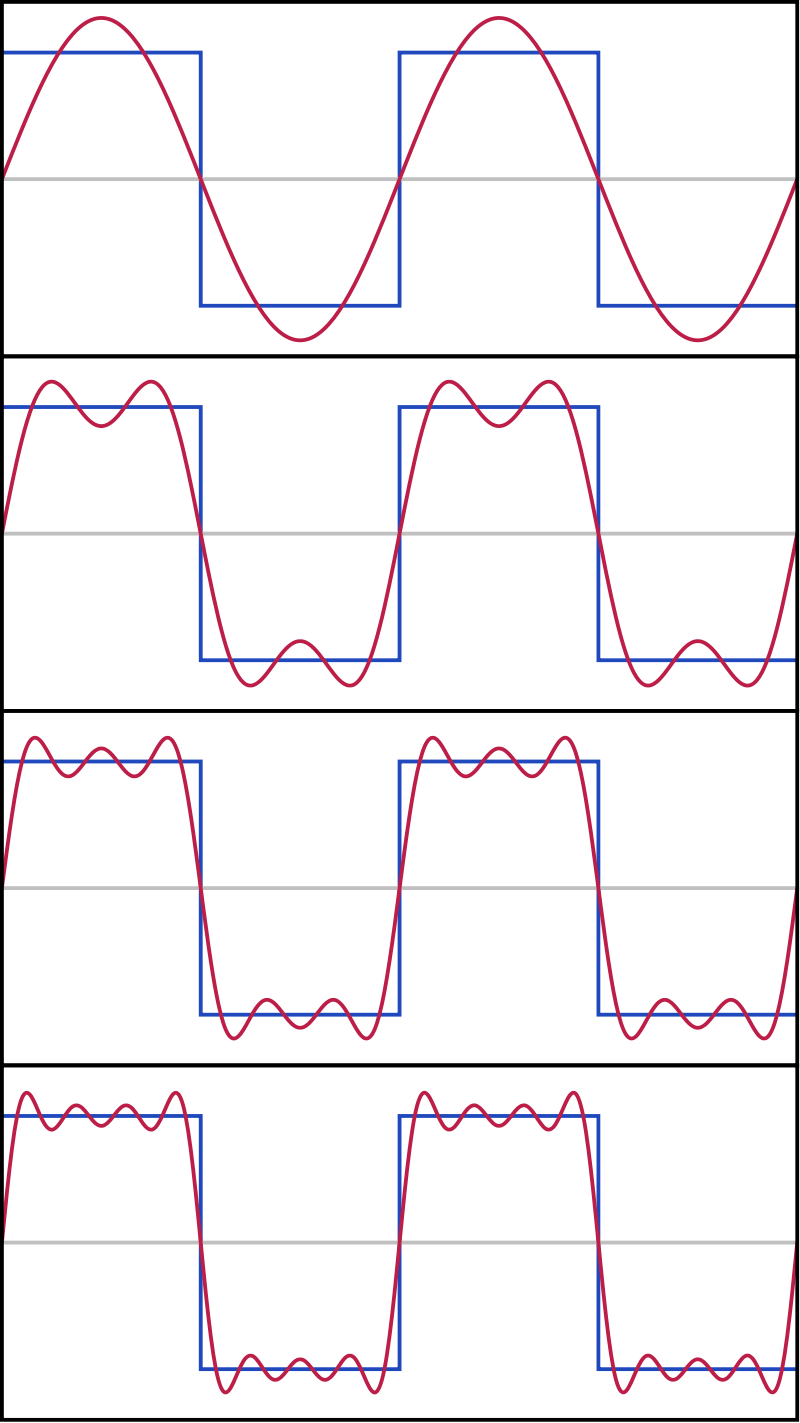
\includegraphics[height=2.5in]{exp/squarewave.png}}
\end{frame}

\begin{frame}
  \frametitle{Spectrum of a Square Wave}

  The Fourier series coefficients of this square wave are
  \begin{align*}
    X_k &= \begin{cases}
      \frac{1}{N_0}\sum_{-N_0/2}^{N_0/2-1} x[n] & k=0\\
      \frac{1}{N_0}\sum_{-N_0/2}^{N_0/2-1} x[n]e^{-j2\pi kn/N_0} & k\ne 0
    \end{cases}\\
    &= \begin{cases}
      \frac{1}{N_0}\sum_{-(L-1)/2}^{(L-1)/2}1 & k=0\\
      \frac{1}{N_0}\sum_{-(L-1)/2}^{(L-1)/2} e^{-j2\pi kn/N_0} & k\ne 0
    \end{cases}
  \end{align*}
\end{frame}

\begin{frame}
  \frametitle{Spectrum of a Square Wave}

  The Fourier series coefficients of this square wave are
  approximately, but not exactly, the same as they would be in the
  continuous-time case:
  \begin{align*}
    X_k&\approx \begin{cases}
      \frac{L}{N_0} & k=0\\
      \frac{\sin(\pi kL/N_0)}{\pi k} & k\ne 0
    \end{cases}
  \end{align*}
  \centerline{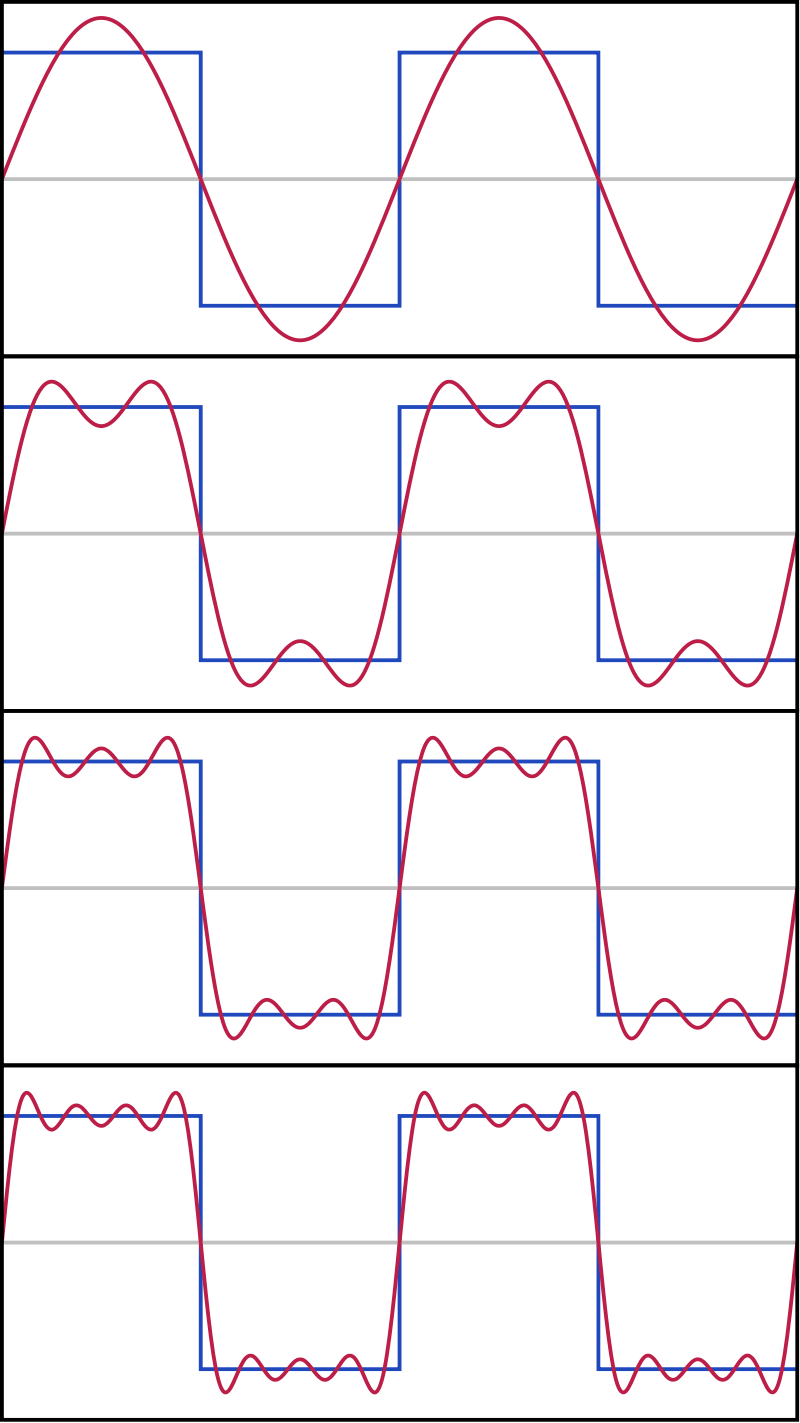
\includegraphics[height=2.5in]{exp/squarewave.png}}
\end{frame}

\begin{frame}
  \frametitle{More about the phase spectrum}
  \centerline{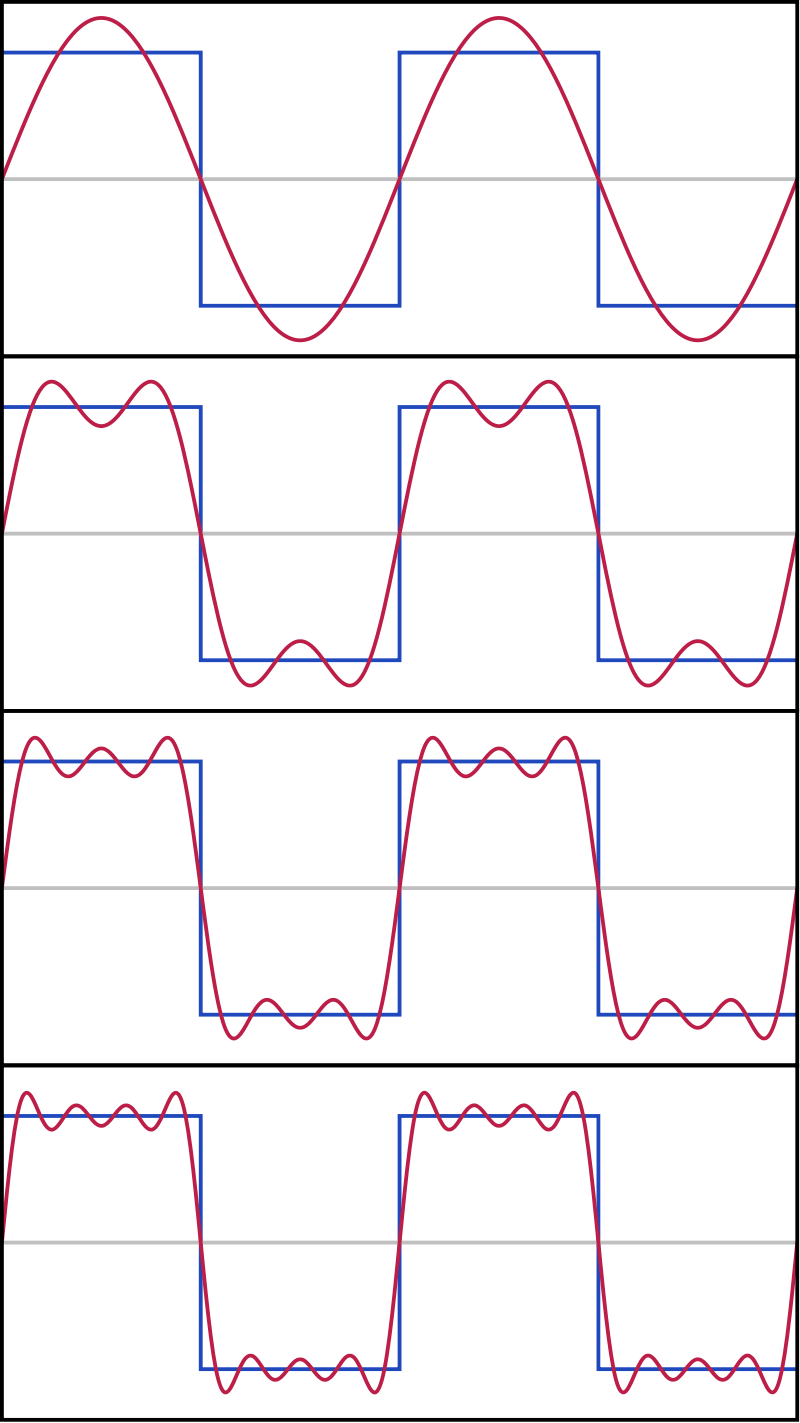
\includegraphics[height=1.5in]{exp/squarewave.png}}
  Notice that, for the phase spectrum of a square wave, the phase
  spectrum is either $\angle X[k]=0$ or $\angle X[k]=\pi$.  That means that the
  spectrum is real-valued, with no complex part:
  \begin{itemize}
  \item {\bf Positive real:} $X[k]=|X[k]|$
  \item {\bf Negative real:} $X[k]=-|X[k]| = |X[k]|e^{j\pi}$
  \end{itemize}
\end{frame}

\begin{frame}
  \frametitle{More about the phase spectrum}
  
  Having discovered that the square wave has a real-valued $X[k]$, we could
  just plot $X[k]$ itself, instead of plotting its magnitude and phase:
  \centerline{\includegraphics[height=2.5in]{exp/squarewave_real.png}}
\end{frame}

\begin{frame}
  \frametitle{Fourier Series and Fourier Transform}

  Notice that, for both the continuous-time and discrete-time Fourier
  series, the square wave has three basic properties:
  \begin{itemize}
  \item $X_0$ is just the average value of $x(t)$.
  \item $X_k$ is (exactly or approximately) $\sin(\pi kL/T_0)/\pi k$.
  \item If the square wave is symmetric in time, then $X_k$ is
    real-valued.
  \end{itemize}
  Now let's see how those properties generalize to the DTFT of a
  non-periodic rectangle.
\end{frame}

%%%%%%%%%%%%%%%%%%%%%%%%%%%%%%%%%%%%%%%%%%%%
\section[Averaging]{The Local Averaging Filters}
\setcounter{subsection}{1}

\begin{frame}
  \frametitle{Local Average Filters}

  Let's go back to the local averaging filter. I want to define two 
  different types of local average: centered, and delayed.
  \begin{itemize}
  \item {\bf Centered local average:} This one averages
    $\left(\frac{L-1}{2}\right)$ future samples,
    $\left(\frac{L-1}{2}\right)$ past samples, and $x[n]$:
    \[
    y_c[n] = \frac{1}{L}\sum_{m=-\left(\frac{L-1}{2}\right)}^{\left(\frac{L-1}{2}\right)} x[n-m]
    \]
  \item {\bf Causal local average:} This one averages $x[n]$ and $L-1$ of its
    past samples:
    \[
    y_d[n] = \frac{1}{L}\sum_{m=0}^{L-1} x[n-m]
    \]
  \end{itemize}
  Notice that $y_d[n] = y_c\left[n-\left(\frac{L-1}{2}\right)\right]$.
\end{frame}

\begin{frame}
  \frametitle{Local Average Filters}

  We can write both of these as filters:
  \begin{itemize}
  \item {\bf Centered local average:}
    \begin{align*}
      y_c[n] &= f_c[n]\ast x[n]\\
      f_c[n] &= \begin{cases} \frac{1}{L}& -\left(\frac{L-1}{2}\right)\le n\le\left(\frac{L-1}{2}\right)\\
        0&\mbox{otherwise}\end{cases}
    \end{align*}
  \item {\bf Causal local average:}
    \begin{align*}
      y_d[n] &= f_d[n]\ast x[n]\\
      f_d[n] &= \begin{cases} \frac{1}{L}& 0\le n\le L-1\\
        0&\mbox{otherwise}\end{cases}
    \end{align*}
  \end{itemize}
\end{frame}

\begin{frame}
  \frametitle{Local Average Filters}
  \centerline{\includegraphics[height=2.5in]{exp/localaveragefilters.png}}
  Notice that $f_d[n]=f_c\left[n-\left(\frac{L-1}{2}\right)\right]$.
\end{frame}  

\begin{frame}
  \frametitle{The relationship between centered local average and delayed local average}

  Notice that $f_d[n]=f_c[n-\frac{L-1}{2}]$.  We can find the
  relationship between their DTFTs using variable substitution, with
  the variable $m=n-\frac{L-1}{2}$:
  \begin{align*}
    F_d(\omega) &= \sum_{n=-\infty}^\infty f_d[n]e^{-j\omega n}\\
    &=\sum_{n=-\infty}^\infty f_c[n-\frac{L-1}{2}]e^{-j\omega n}\\
    &=e^{-j\omega\frac{L-1}{2}}\sum_{m=-\infty}^\infty f_c[m]e^{-j\omega m}\\
    &=e^{-j\omega\frac{L-1}{2}}F_c(\omega)
  \end{align*}
\end{frame}
  
\begin{frame}
  \frametitle{The frequency response of a local average filter}

  Let's find the frequency response of
  \[
  f_d[n] = \begin{cases} \frac{1}{L}& 0\le m\le L-1\\
    0&\mbox{otherwise}\end{cases}
  \]
  The formula is
  \[
  F_d(\omega) = \sum_m f[m]e^{-j\omega m},
  \]
  so,
  \[
  F_d(\omega) = \sum_{m=0}^{L-1} \frac{1}{L}e^{-j\omega m}
  \]
\end{frame}
  
\begin{frame}
  \frametitle{The frequency response of a local average filter}

  \[
  F_d(\omega) = \sum_{m=0}^{L-1} \frac{1}{L}e^{-j\omega m}
  \]
  This is just a standard geometric series,
  \[
  \sum_{m=0}^{L-1} a^m = \frac{1-a^L}{1-a},
  \]
  so:
  \[
  F_d(\omega) = \frac{1}{L}\left(\frac{1-e^{-j\omega L}}{1-e^{-j\omega}}\right)
  \]
\end{frame}

\begin{frame}
  \frametitle{The frequency response of a local average filter}

  We now have an extremely  useful transform pair:
  \[
  f_d[n] = \begin{cases} \frac{1}{L}& 0\le m\le L-1\\
    0&\mbox{otherwise}\end{cases}~~~\leftrightarrow~~~
  F_d(\omega) = \frac{1}{L}\left(\frac{1-e^{-j\omega L}}{1-e^{-j\omega}}\right)
  \]
  Let's attempt to convert that into polar form, so we can find
  magnitude and phase response. Notice that both the numerator and the
  denominator are subtractions of complex numbers, so we might be able
  to use $2j\sin(x)=e^{jx}-e^{-jx}$ for some $x$.  Let's try:
  \begin{align*}
    \frac{1}{L}\left(\frac{1-e^{-j\omega L}}{1-e^{-j\omega}}\right)
    &= \frac{1}{L}\frac{e^{-j\omega L/2}}{e^{-j\omega/2}}
    \left(\frac{e^{j\omega L/2}-e^{-j\omega L/2}}{e^{j\omega/2}-e^{-j\omega/2}}\right)\\
    &= e^{-j\omega\left(\frac{L-1}{2}\right)}\frac{1}{L}
    \left(\frac{2j\sin(\omega L/2)}{2j\sin(\omega/2)}\right)\\
    &= e^{-j\omega\left(\frac{L-1}{2}\right)}\frac{1}{L}
    \left(\frac{\sin(\omega L/2)}{\sin(\omega/2)}\right)
  \end{align*}
\end{frame}
  
\begin{frame}
  \frametitle{Quiz}

  Go to the course web page, and try the quiz!
\end{frame}

\begin{frame}
  \frametitle{The frequency response of a local average filter}

  Now we have $F_d(\omega)$ in almost magnitude-phase form:
  \[
  f_d[n] = \begin{cases} \frac{1}{L}& 0\le m\le L-1\\
    0&\mbox{otherwise}\end{cases}~~~\leftrightarrow~~~
  F_d(\omega)=\left(\frac{\sin(\omega L/2)}{L\sin(\omega/2)}\right)e^{-j\omega\left(\frac{L-1}{2}\right)}
  \]
  By the way, remember we discovered that
  \[
  F_d(\omega)=e^{-j\omega\left(\frac{L-1}{2}\right)}F_c(\omega)
  \]
  Notice anything?
\end{frame}

\begin{frame}
  \frametitle{DTFT of Local Averaging Filters}

  \begin{itemize}
  \item {\bf Centered local average:}
    \begin{align*}
      f_c[n] &= \begin{cases} \frac{1}{L}& -\left(\frac{L-1}{2}\right)\le n\le\left(\frac{L-1}{2}\right)\\
        0&\mbox{otherwise}\end{cases}\\
      F_c(\omega)&=\frac{\sin(\omega L/2)}{L\sin(\omega/2)}
    \end{align*}
  \item {\bf Causal local average:}
    \begin{align*}
      f_d[n] &= \begin{cases} \frac{1}{L}& 0\le n\le L-1\\
        0&\mbox{otherwise}\end{cases}
      F_d(\omega) &=\frac{\sin(\omega L/2)}{L\sin(\omega/2)}e^{-j\omega\left(\frac{L-1}{2}\right)}
    \end{align*}
  \end{itemize}
\end{frame}

%%%%%%%%%%%%%%%%%%%%%%%%%%%%%%%%%%%%%%%%%%%%
\section[Rectangles]{Rectangular Windows}
\setcounter{subsection}{1}

\begin{frame}
  \frametitle{DTFT of Rectangular Window}

  The local summing filter is just a scaled version of the local
  averaging filter. It is commonly called the ``rectangular window,''
  for reasons that we'll explore in future lectures.
  \begin{itemize}
  \item {\bf Centered rectangular window:}
    \begin{align*}
      w_c[n] &= \begin{cases} 1& -\left(\frac{L-1}{2}\right)\le n\le\left(\frac{L-1}{2}\right)\\
        0&\mbox{otherwise}\end{cases}\\
      W_c(\omega)&=\frac{\sin(\omega L/2)}{\sin(\omega/2)}
    \end{align*}
  \item {\bf Causal rectangular window:}
    \begin{align*}
      w_d[n] &= \begin{cases} 1& 0\le n\le L-1\\
        0&\mbox{otherwise}\end{cases}
      W_d(\omega) &=\frac{\sin(\omega L/2)}{\sin(\omega/2)}e^{-j\omega\left(\frac{L-1}{2}\right)}
    \end{align*}
  \end{itemize}
\end{frame}


\begin{frame}
  \frametitle{Dirichlet form}

  Of all four of these signals, the centered rectangular window has
  the simplest DTFT. The textbook calls this signal the ``Dirichlet
  form:''
  \[
  D_L(\omega) = \frac{\sin(\omega L/2)}{\sin(\omega/2)}
  \]
  That is, exactly, the frequency response of a centered rectangular window:
  \[
  d_L[n] = w_c[n] = \begin{cases}
    1 & -\left(\frac{L-1}{2}\right)\le n\le \left(\frac{L-1}{2}\right)\\
    0 & \mbox{otherwise}
  \end{cases}
  \]
\end{frame}

\begin{frame}
  \frametitle{Dirichlet form}

  Here's what it looks like:
  \centerline{\includegraphics[height=2.5in]{exp/dirichletform.png}}
\end{frame}
  
\begin{frame}
  \frametitle{Dirichlet form}

  Since every local averaging filter is based on Dirichlet form, it's
  worth spending some time to understand it better.
  \[
  D_L(\omega) = \frac{\sin(\omega L/2)}{\sin(\omega/2)}
  \]
  \begin{itemize}
  \item It's equal to zero every time $\omega L/2$ is a multiple of $\pi$.  So
    \[
    D_L\left(\frac{2\pi k}{L}\right)  = 0~~\mbox{for all integers}~k~\mbox{except}~k=0
    \]
  \item At $\omega=0$, the value of $\frac{\sin(\omega
    L/2)}{\sin(\omega/2)}$ is undefined, but it's posssible to prove
    that $\lim_{\omega\rightarrow 0}D_L(\omega)=L$.  To make life
    easy, we'll just define it that way:
    \[
    \mbox{DEFINE:}~~D_L(0)=L
    \]
  \end{itemize}
\end{frame}

\begin{frame}
  \frametitle{Dirichlet form}

  Here's what it looks like:
  \centerline{\includegraphics[height=2.5in]{exp/dirichletform.png}}
\end{frame}
  
\begin{frame}
  \frametitle{Local averaging filter}

  Here's what the centered local averaging filter looks like.  Notice that
  it's just $1/L$ times the Dirichlet form:
  \centerline{\includegraphics[height=2.5in]{exp/centeredaveragingfilter.png}}
\end{frame}
  

%%%%%%%%%%%%%%%%%%%%%%%%%%%%%%%%%%%%%%%%%%%%
\section[Summary]{Summary}
\setcounter{subsection}{1}

\begin{frame}
  \frametitle{Summary: DTFTs of Rectangular Windows}
  \begin{itemize}
  \item The {\bf Centered Local Averaging Filter} is $1/L$ times
    the Dirichlet form:
    \[
    f_c[n] = \begin{cases}
      \frac{1}{L} & -\left(\frac{L-1}{2}\right)\le n\le \left(\frac{L-1}{2}\right)\\
      0 & \mbox{otherwise}
    \end{cases}~~~\leftrightarrow~~~
    F_c(\omega)=\frac{\sin(\omega L/2)}{L\sin(\omega/2)}
    \]
  \item The {\bf Causal Local Averaging Filter} is $f_c[n]$, delayed by $\frac{L-1}{2}$ samples:
    \[
    f_d[n] = \begin{cases}
      \frac{1}{L} & 0\le n\le L-1\\
      0 & \mbox{otherwise}
    \end{cases}~~~\leftrightarrow~~~
    F_d(\omega)=\frac{\sin(\omega L/2)}{L\sin(\omega/2)}e^{-j\omega\left(\frac{L-1}{2}\right)}
    \]
  \end{itemize}
\end{frame}


\end{document}
